\chapter{Installation d'Unitex}
\label{chap-install}

Unitex est un système multi-plateformes capable de fonctionner aussi bien sous Win
dows que sous Linux ou MacOS. Ce chapitre décrit l’installation et le lancement d’Unitex
pour chacun de ces systèmes. Il présente également les procédures d’ajout de nouvelles
langues et de désinstallation.

\section{Licences}
\label{section-licences}
\index{LGPL}\index{Licences!LGPL}
Unitex est un logiciel libre. Cela signifie que les sources des programmes sont distribuées avec le
logiciel, et que chacun peut les modifier et les redistribuer. Le code des programmes d’Unitex est
sous licence LGPL (\cite{LGPL}), à l’exception de la bibliothèque de manipulation d’expressions
régulières TRE de Ville Laurikari (\cite{TRE}), qui est sous licence GPL.
La licence LGPL est plus permissive que la licence GPL, car elle permet d’utiliser du code LGPL dans
des logiciels non libres. Du point de vue de l’utilisateur, il n’y a pas de différence, car dans
les deux cas, le logiciel peut être librement utilisé et distribué.


\bigskip
\noindent Toutes les données linguistiques distribuées avec Unitex sont soumises à la licence LGPLLR
\index{LGPLLR} (\cite{LGPLLR}).

\bigskip
\noindent Le texte complet des licences GPL, LGPL et LGPLLR se trouve dans les annexes à la fin de
ce manuel.

\section{Environnement d’exécution Java}
Unitex est composé d’une interface graphique écrite en Java et de programmes externes
écrits en \textit{C/C\kern-.05em\raisebox{.5ex}{++}\kern-.1em}. Ce mélange de langages de 
programmation permet d’avoir une application rapide et portable sous différents systèmes d’exploitation.


\bigskip
\noindent Afin de pouvoir utiliser l’interface graphique, il faut préalablement installer
un environnement d’exécution, communément appelé machine virtuelle \index{Java virtual machine} ou
JRE\index{JRE} (Java Runtime Environment\index{Java Runtime Environment}).

\bigskip
\noindent Pour fonctionner en mode graphique, Unitex nécessite une version 1.6 (ou plus récente)
de Java. Si vous avez une version trop ancienne de Java, Unitex se bloquera après que vous
ayez choisi votre langue de travail.


\bigskip
\noindent Vous pouvez télécharger librement la machine virtuelle correspondant à votre 
système d’exploitation sur le site de Sun Microsystems (\cite{site-java}) à l’adresse suivante : 
\url{http://java.sun.com}.

\bigskip
\noindent Si vous travaillez sous Linux ou MacOS, ou si vous
utilisez une version de Windows gérant des comptes personnels pour les utilisateurs, il vous
faudra demander à votre administrateur système d’installer Java.



\section{Installation sous Windows}
\index{Installation sous Windows}
    Si vous désirez installer Unitex sur une machine Windows multi-utilisateurs, il est pré-
férable de demander à votre administrateur de le faire. Si vous êtes l’utilisateur unique de
votre machine, vous pouvez effectuer l’installation vous-même.

\bigskip
\noindent Décompressez le fichier \index{Fichier!\verb+Unitex3.0.zip+} \verb+Unitex3.0.zip+
(vous pouvez télécharger ce fichier à l’adresse suivante : \url{http://www-igm.univ-mlv.fr/~unitex})
dans un répertoire \verb+Unitex3.0+ que vous aurez préalablement créé, de préférence dans le répertoire  \verb+Program Files+.

\bigskip
\noindent Après la décompression, le répertoire \verb+Unitex3.0+ contient plusieurs
sous-répertoires dont un nommé \verb+App+. Ce dernier répertoire contient un fichier nommé
\verb+Unitex.jar+\index{Fichier!\verb+Unitex.jar+}.                                                            Ce fichier est l’exécutable Java qui lance l’interface graphique. Il vous suffit de double-cliquer
dessus pour lancer le programme.
Pour faciliter le lancement du programme, il est conseillé de créer un raccourci vers ce fichier sur le bureau.


\section{Installation sous Linux}
\index{Installation sous Linux}
Pour installer Unitex sous Linux et MacOS, il est recommandé d’être administrateur système. Décompressez le fichier \verb+Unitex3.0.zip+ dans un répertoire nommé
\verb+Unitex+, au moyen de la commande suivante :


\bigskip \noindent \verb$unzip Unitex3.0.zip -d Unitex$

\bigskip
\noindent Placez-vous ensuite dans le répertoire \verb|Unitex/Src/C++/build|                                     , et lancez la compilation des
programmes au moyen de la commande :


\bigskip \verb+make install+

\bigskip
\noindent ou si avez un ordinateur 64 bits avec la commande :
 
\bigskip \verb+make install 64BITS=yes+

\bigskip
\noindent Créez ensuite un alias sur le modèle suivant :

\bigskip \verb$alias unitex='cd /..../Unitex/App/ ; java -jar Unitex.jar'$


\section{Installation sous MacOS X}
\index{Installation sous MacOS X}
\label{section-macos-install}
\noindent NOTE: ce court tutoriel va vous expliquer comment installer et exécuter Unitex sous Mac OS
X. Vos questions, commentaires, suggestions,
corrections sont plus que bienvenus.
\noindent Contact: \url{cedrick.fairon@uclouvain.be}

\bigskip
\noindent Une version officielle de Java 1.6 existe pour MacOS X 10.5, 64-bit Intel 
(Core 2 Duo), mais il n'y a pas de solution officielle pour les anciens OS X (10.4 ou plus anciens),
PowerPC et 32-bit Intel (Core Duo). Ainsi,
 si vous avez OS X 10.5, un MacOS 64-bit Intel, il vous suffit de vous procurer
	la JRE 1.6. Apple. Le seul problème est que cette version ne démarre pas par défaut.
	Voir section ``Java for Mac OS X 10.5 Update 2'', à \url{http://developer.apple.com/java/}


\noindent\textbf{Comment savoir si mon processeur est un 32 ou un 64 bits ?}

\noindent Dans le menu Apple, cliquez sur "About this Mac". Si vous voyez quelquechose comme:
"Processor : x.xx Ghz Intel Core Duo", votre processeur est un 32 bits.

\bigskip
\noindent Si vous voyez "Processeur: x.xx Ghz Intel Core 2 Duo", ou si votre
processeur est de type Intel (comme Xeon), alors vous avez un processeur 64 bits.

\subsection{Utiliser Apple Java 1.6 runtime}
\bigskip\index{Utiliser Apple Java 1.6 runtime}
\noindent Si vous utilisez Mac OS X 10.5 (ou ultérieur) sur des processeurs Intel 64 bits, vous pouvez simplement utiliser le Java 1.6 d'Apple. Vous pouvez l'obtenir à partir de \url{http://www.apple.com/support/downloads/javaformacosx105update1.html}.

\noindent Vous pouvez aller dans Application -> Utilities -> Java Preferences pour vérifier la présence  de "Java SE 6" dans la liste "Java Applications".


\subsubsection{Option 1 : modifier le runtime par défaut pour Java Applications}
\noindent Si vous n'utilisez pas une autre application Java qui a besoin de Java 1.5, vous pouvez
simplement mettre "Java SE 6" en haut de la liste «Applications Java" dans Utilitaire de préférence
Java.
\subsubsection{Option 2 : Créer un alias pour lancer Java 1.6}
\noindent Si vous ne voulez pas modifier les paramètres globaux de Java, vous pouvez créer un alias

\bigskip
\noindent \verb+alias jre6="/System/Library/Frameworks/JavaVM.framework/Versions/+
\noindent \verb+1.6/Commands/java"+
   
\bigskip
\noindent \verb+jre6 -jar Unitex.jar+

\bigskip
\noindent Ensuite lancer Unitex depuis un terminal.

%\subsection{SoyLatte}

%\subsection{Comment compiler les programmes les C++ Unitex sur un ordinateur Macintosh}


\subsection{Comment rendre tous les fichiers visibles sur Mac OS}
\noindent Voir
\url{http://www.macworld.com/article/51830/2006/07/showallfinder.html}.

\bigskip
\noindent Ou essayez tout de suite... Tapez: 

\bigskip
\verb+defaults write com.apple.Finder AppleShowAllFiles ON+

\bigskip
\noindent Ensuite redémarrez le Finder:

\bigskip
\verb+killall Finder+

\begin{figure}[!h]
\begin{center}
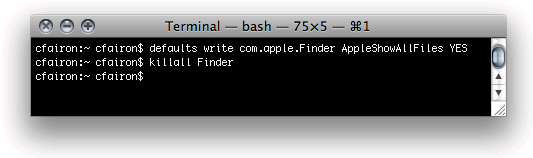
\includegraphics[width=12cm]{resources/img/fig-mac6.png}
\caption{Redémarrez le Finder\label{fig-mac6}}
\end{center}
\end{figure}

\bigskip
\noindent Pour revenir à la configuration d'origine, tapez: 

\bigskip
\verb+defaults write com.apple.Finder AppleShowAllFiles OFF+


\section{Première utilisation}
Si vous travaillez sous Windows, le programme vous demandera de choisir un répertoire personnel
\index{Répertoire personnel} de travail, que vous pourrez changer ultérieurement dans
"Info>Preferences...>Di-rectories". Pour créer un répertoire, cliquez sur l’icône représentant un
dossier (voir figure \ref{fig-creation-personal-directory}).

\bigskip
\noindent Sous Linux et MacOS, le programme créera automatiquement un répertoire
\verb+/unitex+ dans votre répertoire \verb+$HOME+. Ce répertoire vous permettra de stocker vos
données personnelles. 
Pour chaque langue que vous utiliserez, le programme copiera l’arborescence de la langue dans votre
répertoire personnel,
à l’exception des dictionnaires. Vous pourrez ainsi modifier à votre guise votre copie des données
sans risquer d’endommager les données du système.



\begin{figure}[h]
\begin{center}
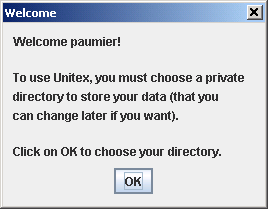
\includegraphics[width=6.3cm]{resources/img/fig1-1.png}
\caption{Première utilisation sous Windows}
\end{center}
\end{figure}

\begin{figure}[h]
\begin{center}
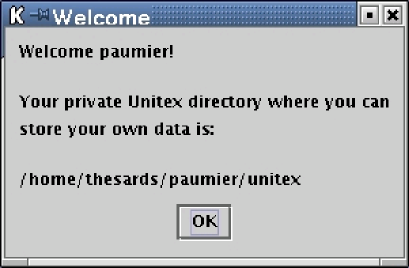
\includegraphics[width=7cm]{resources/img/fig1-2.png}
\caption{Première utilisation sous Linux}
\end{center}
\end{figure}

\begin{figure}[h]
\begin{center}
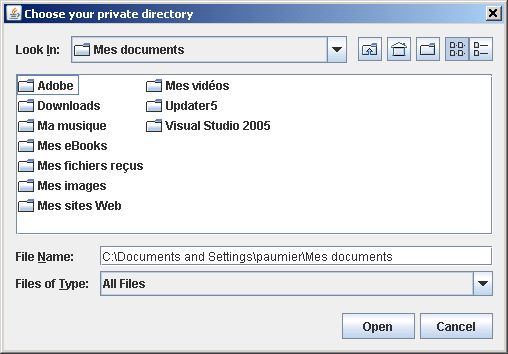
\includegraphics[width=13cm]{resources/img/fig1-3.png}
\caption{Création du répertoire de travail personnel
\label{fig-creation-personal-directory}}
\end{center}
\end{figure}



\section{Ajout de nouvelles langues}
\index{Ajout de nouvelles langues}

\bigskip
\noindent Il y a deux manières d’ajouter des langues. Si vous désirez ajouter une nouvelle langue
accessible à tous les utilisateurs, il vous faut copier le répertoire correspondant à cette langue
dans le répertoire Unitex du système, ce qui nécessite d’avoir les droits d’accès à ce répertoire
(il vous faudra peut-être demander à votre administrateur système de le faire).
En revanche, si la langue ne concerne qu’un seul utilisateur, celui-ci peut copier le répertoire
en question dans son répertoire personnel. Il pourra ainsi travailler sur cette langue, sans
qu’elle soit proposée aux autres utilisateurs.



\section{Désinstallation}
Quel que soit le système sous lequel vous travaillez, il vous suffit de supprimer le répertoire
\verb+Unitex+ pour effacer tous les fichiers du système. Sous Windows, vous devrez ensuite supprimer
le raccourci vers \verb+Unitex.jar+ \index{Fichier!\verb+Unitex.jar+} si vous en avez créé un ;
même chose sous Linux ou MacOS si vous avez créé un alias.


\section{Unitex pour les développeurs}
\label{section-unitex-developpers}
Si vous êtes programmeur, cela peut vous intéresser de lier votre code avec les sources C++
d'Unitex. Pour faciliter cette opération, vous pouvez compiler Unitex en tant que librairie
dynamique qui contient toutes les fonctions Unitex functions, sauf \verb+main+s, bien sûr. Sous
Linux/MacOS, tapez:

\bigskip
\verb+make LIBRARY=yes+

\bigskip
\noindent et vous obtiendrez une librairie nommée \verb+libunitex.so+. Si vous souhaitez produire 
DLL Windows nommée \verb+unitex.dll+, utilisez les commandes suivantes:

\bigskip
Windows: \verb+make SYSTEM=windows LIBRARY=yes+

Cross-compilation avec mingw32: \verb+make SYSTEM=mingw32 LIBRARY=yes+

\bigskip
\noindent dans tous les cas, vous obtiendrez aussi un programme nommé
\verb+Test_lib+(\verb+.exe+). Si tout a bien fonctionné, ce programme devrait afficher l'écran
suivant:

\begin{verbatim}
Expression converted.
Reg2Grf exit code: 0

#Unigraph
SIZE 1313 950
FONT Times New Roman:  12
OFONT Times New Roman:B 12
BCOLOR 16777215
FCOLOR 0
ACOLOR 12632256
SCOLOR 16711680
CCOLOR 255
DBOXES y
DFRAME y
DDATE y
DFILE y
DDIR y
DRIG n
DRST n
FITS 100
PORIENT L
#
7
"<E>" 100 100 1 5
"" 100 100 0
"a" 100 100 1 6
"b" 100 100 1 4
"c" 100 100 1 6
"<E>" 100 100 2 2 3
"<E>" 100 100 1 1
\end{verbatim}
